\begin{subfigure}{5em}
	\centering
	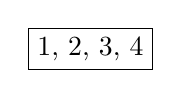
\begin{tikzpicture}
		\node[draw] (root) {1, 2, 3, 4};
	\end{tikzpicture}
	\caption*{One Node}
\end{subfigure}
\begin{subfigure}{7em}
	\centering
	\begin{tikzpicture}[node distance=0.25]
		\node[draw] (leaf1) {1, 2};
		\node[draw] (leaf2) [right=of leaf1] {3, 4, 5};
		\coordinate (center) at ($ (leaf1) !.5! (leaf2) $);
		\node[draw] (root) [above=0.5 of center] {2, 5};
		\draw (root) -- (leaf1);
		\draw (root) -- (leaf2);
	\end{tikzpicture}
	\caption*{After First Split}
\end{subfigure}
\begin{subfigure}{14em}
	\centering
	\begin{tikzpicture}[node distance=0.25]
		\node[draw] (leaf1) {1, 2};
		\node[draw] (leaf2) [right=of leaf1] {3, 4};
		\node[draw] (leaf3) [right=of leaf2] {5, 6};
		\node[draw] (leaf4) [right=of leaf3] {7, 8, 9, 10};
		\coordinate (center) at ($ (leaf2) !.5! (leaf3) $);
		\node[draw] (root) [above=0.5 of center] {2, 4, 6, 10};
		\draw (root) -- (leaf1);
		\draw (root) -- (leaf2);
		\draw (root) -- (leaf3);
		\draw (root) -- (leaf4);
	\end{tikzpicture}
	\caption*{Before Second Split}
\end{subfigure}
\begin{subfigure}{16em}
	\centering
	\begin{tikzpicture}[node distance=0.25]
		\node[draw] (leaf1) {1, 2};
		\node[draw] (leaf2) [right=of leaf1] {3, 4};
		\node[draw] (leaf3) [right=of leaf2] {5, 6};
		\node[draw] (leaf4) [right=of leaf3] {7, 8};
		\node[draw] (leaf5) [right=of leaf4] {9, 10, 11};
		\coordinate (center1) at ($ (leaf4) !.5! (leaf5) $);
		\coordinate (center2) at ($ (leaf2) !.5! (leaf3) $);
		\node[draw] (inner1) [above=0.5 of center1] {8, 11};
		\node[draw] (root) [above=1 of center2] {2, 4, 6, 11};
		\draw (root) -- (leaf1);
		\draw (root) -- (leaf2);
		\draw (root) -- (leaf3);
		\draw (root) -- (inner1);
		\draw (inner1) -- (leaf4);
		\draw (inner1) -- (leaf5);
	\end{tikzpicture}
	\caption*{After Second Split}
\end{subfigure}
\begin{subfigure}{9em}
	\centering
	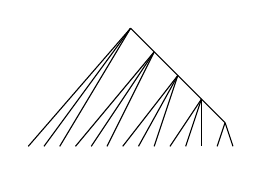
\begin{tikzpicture}[xscale=-0.2, yscale=0.3]
		\draw (1.5, 1) -- (1, 0);
		\draw (1.5, 1) -- (2, 0);
		\foreach \i in {2,...,5} {
			\draw ({\i*1.5}, \i) -- ({(\i-1)*1.5}, \i-1);
			\draw ({\i*1.5}, \i) -- ({3*(\i-1)}, 0);
			\draw ({\i*1.5}, \i) -- ({3*(\i-1)+1}, 0);
			\draw ({\i*1.5}, \i) -- ({3*(\i-1)+2}, 0);
		}
	\end{tikzpicture}
	\caption*{Overall Pattern}
\end{subfigure}
